\documentclass[12pt]{article}
\parindent=0.25in

\setlength{\oddsidemargin}{0pt}
\setlength{\textwidth}{440pt}
\setlength{\topmargin}{0in}
\usepackage{amssymb}
\usepackage{amsfonts}
\usepackage{amsmath}
\usepackage{cancel}
\usepackage{latexsym}
\usepackage[center]{subfigure}
\usepackage{epsfig}
\usepackage{3952}
\usepackage{3952-thm}
\usepackage{pstricks,pst-node,pst-tree}
\usepackage{soul, xcolor}
\usepackage{bbold}
\usepackage[backref, colorlinks,citecolor=blue,bookmarks=true]{hyperref}  

\pagestyle{headings}    % Go for customized headings

\newcommand{\handout}[5]{
   \noindent
   \begin{center}
   \framebox{
      \vbox{
    \parbox[t]{4in} {\bf #1 } \vspace{3mm}  {\hfill \bf #2 }
       \vspace{2mm}
       \hbox to 6.00in { {\Large \hfill #5  \hfill} }
       \vspace{1mm}
       \hbox to 6.00in { {\it #3 \hfill #4} }
      }
   }
   \end{center}
   \vspace*{1mm}
}

\hypersetup{linkcolor=magenta}

\begin{document}

\handout{MATH 3952 (Undergraduate Seminar): Quantum Information Theory}{Spring 2024}
{Organizer: Patrick Lei; Presenter: Francesco Stern}
{Scribe: Mark Chen}{Lecture 5, Talk 2: February 26, 2024}

\thispagestyle{plain}
% \setcounter{section}{-1}
\section*{Chapter 5: Entanglement (Ctd.)}
\section{Quantum Teleportation}
The circuit representation is:
\begin{center}
    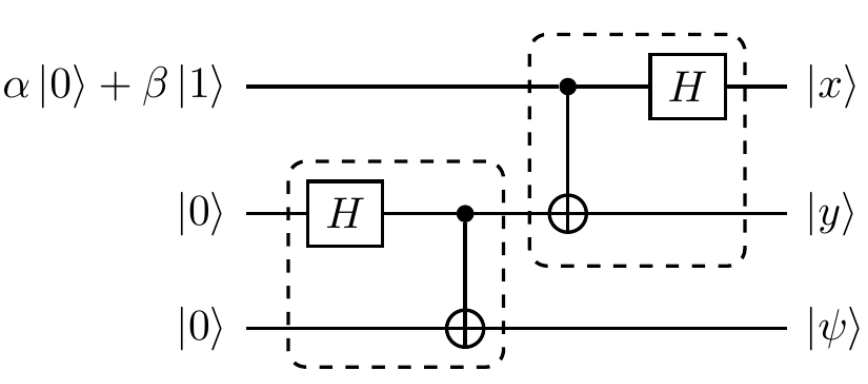
\includegraphics[width = 20em]{images/5.jpg}
\end{center}

\noindent Particularly, Alice has an unknown $$
\Ket{\psi} = \alpha\Ket{0} + \beta \Ket{1}
$$ and wants to somehow let the distant Bob to know what this state is. And the idea for doing so is known as the quantum teleportation.\\

\noindent Based on the circuit, it is not hard to do the normal things and realize that it represents the following transformations (up to after the first dashed box): \begin{equation}
\begin{aligned}
(\alpha \Ket{0} + \beta \Ket{1})\otimes \Ket{0}\otimes \Ket{0}
    &\overset{\mathbb{1}\otimes H\otimes \mathbb{1}}{\mapsto}(\alpha \Ket{0} + \beta \Ket{1})\otimes \prt{\frac{1}{\sqrt{2}}(\Ket{0} + \Ket{1})\otimes \Ket{0}} = (\alpha \Ket{0} + \beta \Ket{1})\otimes \frac{1}{\sqrt{2}}(\Ket{00} + \Ket{10})\\
    &\overset{\mathbb{1}\otimes \text{c-}\NOT}{\mapsto}(\alpha \Ket{0} + \beta \Ket{1})\otimes \frac{1}{\sqrt{2}}(\Ket{00} + \Ket{11})\\
\end{aligned}
\end{equation}

\begin{lemma}
$(\alpha \Ket{0} + \beta \Ket{1})\otimes \frac{1}{\sqrt{2}}(\Ket{00} + \Ket{11}) = (\alpha \Ket{0} + \beta \Ket{1})\otimes \Phi^+$ can be expanded into the following form: $$
2(\alpha \Ket{0} + \beta \Ket{1})\otimes \Phi^+ = \Phi^+\otimes(\alpha\Ket{0} + \beta\Ket{1}) + \Psi^+\otimes(\alpha\Ket{1} + \beta\Ket{0}) + \Phi^-\otimes(\alpha\Ket{0} - \beta\Ket{1}) + \Psi^-\otimes(\alpha\Ket{1} - \beta\Ket{0})
$$
\end{lemma}
\begin{proof}
First of all, both sides have a factor of $\frac{1}{\sqrt{2}}$, so let's exclude that. Secondly, we expand by distributivity of $\otimes$:
$$
\begin{aligned}
\text{RHS}=
    &(\Ket{00} + \Ket{11})\otimes (\alpha\Ket{0} + \beta\Ket{1})\\
    &+(\Ket{01} + \Ket{10})\otimes (\alpha\Ket{1} + \beta\Ket{0})\\
    &+(\Ket{00} - \Ket{11})\otimes (\alpha\Ket{0} - \beta\Ket{1})\\
    &+(\Ket{01} - \Ket{10})\otimes (\alpha\Ket{1} - \beta\Ket{0})\\
    =
    &\alpha\Ket{000} + \beta\Ket{001} +  \alpha\Ket{110} +  \beta\Ket{111}\\
    &+  \alpha\Ket{011} +  \beta\Ket{010} + \alpha\Ket{101} + \beta\Ket{100}\\
    &+ \alpha\Ket{000} - \beta\Ket{001} -  \alpha\Ket{110} +  \beta\Ket{111}\\
    &+  \alpha\Ket{011} -  \beta\Ket{010} - \alpha\Ket{101} + \beta\Ket{100}\\
    =
    &\alpha\Ket{000} + \beta\Ket{111}\\
    &+ \alpha\Ket{011} + \beta\Ket{100}\\
    &+ \alpha\Ket{000} + \beta\Ket{111}\\
    &+ \alpha\Ket{011} + \beta\Ket{100}\\
    =
    &2\prt{\alpha\Ket{000} + \alpha\Ket{011} + \beta\Ket{100} + \beta\Ket{111}}\\
    =
    &\text{LHS}
\end{aligned}
$$
\end{proof}

\noindent Now, we continue along the circuit based off of (1):
\begin{equation}
\begin{aligned}
(\alpha \Ket{0} + \beta \Ket{1})\otimes \Ket{0}\otimes \Ket{0}
    \overset{\mathbb{1}\otimes \text{c-}\NOT}{\mapsto}
    &(\alpha \Ket{0} + \beta \Ket{1})\otimes \frac{1}{\sqrt{2}}(\Ket{00} + \Ket{11})\\
    &=(\alpha \Ket{0} + \beta \Ket{1})\otimes \Phi^+\\
    &= \frac{1}{2}\big[\Phi^+\otimes(\alpha\Ket{0} + \beta\Ket{1}) + \Psi^+\otimes(\alpha\Ket{1} + \beta\Ket{0})\\
    &\hspace{.5cm}+ \Phi^-\otimes(\alpha\Ket{0} - \beta\Ket{1}) + \Psi^-\otimes(\alpha\Ket{1} - \beta\Ket{0})\big]\\
    \overset{\text{c-}\NOT\otimes \mathbb{1}}{\mapsto}
    &\frac{1}{2}\big[(\Ket{00} + \Ket{10})\otimes(\alpha\Ket{0} + \beta\Ket{1})\\
    &+ (\Ket{01} + \Ket{11})\otimes(\alpha\Ket{1} + \beta\Ket{0})\\
    &+ (\Ket{00} - \Ket{10})\otimes(\alpha\Ket{0} - \beta\Ket{1})\\
    &+ (\Ket{01} - \Ket{11})\otimes(\alpha\Ket{1} - \beta\Ket{0})\big]
\end{aligned}
\end{equation}
Notice how, now, the first two bits are no longer inseparable, so we further (2), so the basis we need are just $\{\Ket{00}, \Ket{01}, \Ket{10}, \Ket{11}\}$ to fully describe the RHS, now:
$$
\text{RHS} \mapsto \Ket{00}\otimes (\alpha\Ket{0} + \beta\Ket{1})+\Ket{01}\otimes (\alpha\Ket{1} + \beta\Ket{0}) +\Ket{10}\otimes (\alpha\Ket{0} - \beta\Ket{1}) +\Ket{11}\otimes (\alpha\Ket{1} - \beta\Ket{0})
$$

\noindent So, looking at the circuit, once we perform the standard measurements and figure observe $\Ket{x}$ and $\Ket{y}$, we can know \underline{what transformation to apply to restore $\Ket{\psi}$}. Particularly: 
\begin{table}[]
    \centering
    \begin{tabular}{ccc}
    $\Ket{xy}$  & & $U$ on the third qubit \\
    \hline
    $\Ket{00}$ & $\implies$ & $\mathbb{1}$ \\
    $\Ket{01}$ & $\implies$ & $X$ \\
    $\Ket{10}$ & $\implies$ & $Z$ \\
    $\Ket{11}$ & $\implies$ & $XZ$ \\
\end{tabular}
\caption{Transformation Based on Bell Measurements}
\label{table:how-to-recover-third-qubit}
\end{table}

\noindent So, applying the corresponding $U$ transformation onto the third qubit restores the $\Ket{\psi}$ for us!

\begin{example}
Consider the following set-up. Qubit $1$ is in a particular state, and Bob came to collect it for a certain experiment. However, by mistake, he took qubit $3$ instead. Qubits $2$ and $3$ are entangled. How does Alice let Bob know by quantum teleportation the state of qubit $1$?
\begin{center}
    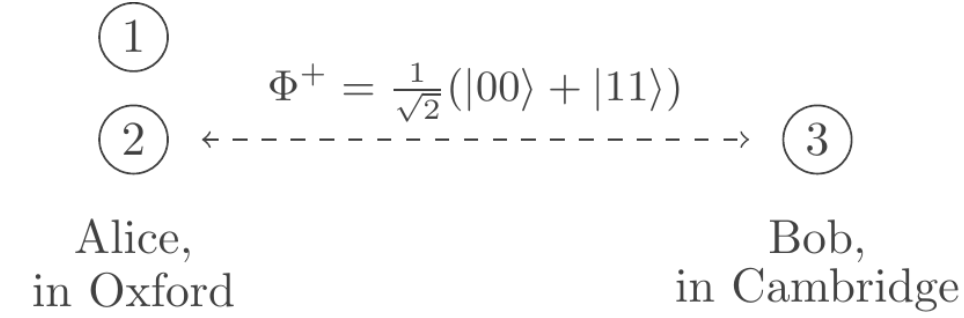
\includegraphics[width = 20em]{images/6.jpg}
\end{center}

\noindent \textbf{Answer:} Alice performs \textbf{Bell measurements} on qubits $1$ and $2$, and then transmit the two bits $\Ket{xy}$ that she observes to Bob. Then, based on table \ref{table:how-to-recover-third-qubit}, Bob can perform the corresponding \textbf{unitary operation} to recover $\Ket{\psi}$. \hl{The communication complexity is $2$ bits} (for $\Ket{xy}$)!
\end{example}

\begin{remark}
Notice that there is no cloning allowed (which we will talk about in the next section). So, by performing the Bell measurement on the first two qubits, the state of the first qubit is necessarily destroyed.
\end{remark}

\section{No-Cloning and Other No-Go Theorem}
It is clearly the case that $\Ket{x0}$ through the c-$\NOT$ gate when $x$ is a single bit gets you $\Ket{xx}$ in the output (just think about a most basic c-$\NOT$ gate).

\noindent Does it have the same property for $\Ket{\psi} = \alpha \Ket{0} + \beta\Ket{1}$ (i.e. a superposition)?

\begin{proposition}
The answer to the question is NO!
\end{proposition}
\begin{proof}
Let's start with $\Ket{\psi}\Ket{0}$, which really is $$
\Ket{\psi}\Ket{0} = (\alpha \Ket{0} + \beta \Ket{1})\Ket{0} = \alpha \Ket{00} + \beta \Ket{10}\overset{\text{c-}\NOT}{\mapsto}\alpha \Ket{00} + \beta \Ket{11}
$$

\noindent However, if we assume ``cloning", then the output should be $$
\Ket{\psi} \Ket{\psi} = (\alpha \Ket{0} + \beta \Ket{1})(\alpha \Ket{0} + \beta \Ket{1}) = \alpha^2\Ket{00} + \beta\alpha\Ket{10} + \alpha\beta\Ket{01} + \beta^2\Ket{11}
$$

\noindent It should be clear that $$
\Ket{\psi}\Ket{0} = \Ket{\psi} \Ket{\psi}\iff (\alpha = 0\text{ and }\beta = 1)\text{ or }(\alpha = 1\text{ and }\beta = 0)
$$

\noindent So, generally, the c-$\NOT$ circuit doesn't get a cloning of states.
\end{proof}

\begin{theorem}\label{thm:no-clone}
It is impossible to clone a general, unknown quantum state.
\end{theorem}
\begin{proof}
Suppose to the contrary that we do have such a unitary operation that allows the following transformation in general (so we can require $\psi$ and $\phi$ to be states that are neither \underline{identical} nor \underline{orthogonal}, i.e. $\bk{\psi}{\phi} \neq 0,1$) $$
\begin{aligned}
\Ket{\psi}\Ket{0}\Ket{W}
    &\mapsto \Ket{\psi}\Ket{\psi}\Ket{W'}\\
\Ket{\phi}\Ket{0}\Ket{W}
    &\mapsto \Ket{\phi}\Ket{\phi}\Ket{W''},
\end{aligned}
$$ where $\Ket{W}$ describes states of everything else in the environment to start with.\\

\noindent Since, again, all physically admissible mappings are unitary, we can require that the inner products to be preserved, so $$
\begin{aligned}
\Bra{W}\Bra{0}\bk{\psi}{\phi}\Ket{0}\Ket{W}
    &= \Bra{W'}\Bra{\psi}\bk{\psi}{\phi}\Ket{\phi}\Ket{W''}\\
\bk{\psi}{\phi}\Bra{W}\underset{1\text{, identical}}{\underbrace{\bk{0}{0}}}\Ket{W}
    &= \bk{\psi}{\phi}\Bra{W'}\bk{\psi}{\phi}\Ket{W''}\\
\bk{\psi}{\phi}\underset{1\text{, identical}}{\underbrace{\bk{W}{W}}}
    &= \bk{\psi}{\phi}^2\bk{W'}{W''}\\
\bk{\psi}{\phi}
    &= \bk{\psi}{\phi}^2\bk{W'}{W''}.
\end{aligned}
$$ Notice that the LHS and RHS are equal $\iff \bk{\psi}{\phi} = 0$ or $1$, which we have chose to exclude. So, $$
\bk{\psi}{\phi} \neq \bk{\psi}{\phi}^2\bk{W'}{W''},
$$ which is a contradiction to the above equality. So, it is impossible for a general cloning machine to exist for unknown quantum states.
\end{proof}

\begin{remark}
Again, because of theorem \ref{thm:no-clone}, we are sure that, during quantum teleportation, the original state must therefore be destroyed, or otherwise we would be producing a clone of an unknown quantum state.\\

\noindent This no-cloning property has many interesting applications, one of which being quantum cryptography.
\end{remark}

\subsection{Other No-Go Theorems}
Broadly, the no-cloning theorem is one of the many such ``no-go theorems" about quantum computing. We will list the others, but not discuss in details:
\begin{itemize}
    \item \textbf{(No-Teleportation)} Teleportation here means classical teleportation. Particularly, it means that an arbitrary quantum state cannot be entirely expressed with classical information, so as to say that the process of converting quantum information to classical information in irreversible.
    \begin{proof}
        Assume this is possible, then we can simply convert quantum information to classical information, clone the classical information, and then convert it back to quantum information. This process would give us a quantum cloning machine, which we have shown to be impossible.
    \end{proof}
    \item \textbf{(No-Broadcasting)} Given a single copy of the quantum state, it is impossible to share with two or more parties.
    \begin{proof}
        If we cannot copy a quantum state, then we cannot share it with multiple parties. More formally, the proof involves \textbf{non-pure states} which require the language of \textbf{density operators} (see chapter 8).
    \end{proof}

    Notice that, using superbroadcasting [\href{https://arxiv.org/pdf/quant-ph/0506251.pdf}{AMP'18}], this would be unexpected: given four copies of an input state, we can actually broadcast six copies!
    \item \textbf{(No-Deleting)} Given two copies of an arbitrary quantum state, it is impossible to delete one.

    \begin{proof}
    Something that people may say about what's special about quantum computing is in \hl{its reversibility, which is a fact dual with all its operations being unitary operators}.
    
    In this sense, we can see deleting as going the reverse time direction of copying (if we can delete a copy, that means in the reverse direction of the deletion, we would have been able to clone a copy -- which can't be the case)
    \end{proof}

    More formally, no-deleting is saying: Given an unknown state $\Ket{\psi}$, there is no \textbf{isometry} (to be defined in chapter 9.3) such that $$
    V: \Ket{\psi}\Ket{\psi}\Ket{W}\mapsto \Ket{\psi}\Ket{0}\Ket{W'},
    $$ which is clearly just the reverse of the impossible ``universal cloning machine", so \hl{a ``universal deleting machine" is impossible as well} (also, not unlike cloning, there are several specific cases where deleting would work, like orthogonal states as they would behave a lot like classical bits).
    \item \textbf{(No-Communication}) An entangled state cannot be used to transmit information by measurement of a subsystem.

    \begin{example}[Einstein's 1947 ``spooky action as a distance"]
        Suppose $\frac{1}{\sqrt{2}}(\Ket{00} + \Ket{11})$, then it seems like we can transmit information instantaneously regardless of distance by measuring subsystem $\HHH_A$ which would cause the state of subsystem $\HHH_B$ to collapse. However, this is not useful, because the state that the local system collapses to is truly random, meaning that the local observer has no control over what is being sent. In other words, \hl{if one wants to leverage this instantaneous communication, one can send no better than truly random bits}.
    \end{example}

    \begin{remark}
        Notice that we can actually prove no-cloning from no-communication, meaning the latter is a stronger phenomenon.
    \end{remark}
    \item \textbf{(No-Hiding)} Quantum information cannot be lost, even through decoherence.

    This is related to no-deletion and shows quantum system's robustness. We will see in chapter 13 about ``quantum noises." But, in situations like those, when quantum information is ``lost" through decoherence, it actually merely moves into the subspace corresponding to the environment (kinda like how energy is lost through friction as heat).

    This is also interesting to physicists as it relates to \href{https://en.wikipedia.org/wiki/Black_hole_information_paradox}{black hole information paradox}.
\end{itemize}

\section{Controlled-Phase and Controlled-U}
\begin{definition}[Controlled-Phase, c-$P_\varphi$]
Like controlled-$\NOT$ we have the following representations:
\begin{itemize}
    \item \textbf{(Matrix)} $$
    \begin{bmatrix}
        1 & 0 & \vline & 0 & 0 \\
        0 & 1 & \vline & 0 & 0 \\
        \hline
        0 & 0 & \vline & 1 & 0 \\
        0 & 0 & \vline & 0 & e^{i\varphi} \\
    \end{bmatrix}
    $$
    \item \textbf{(Circuit)}
    \begin{center}
        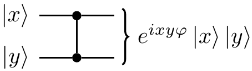
\includegraphics[width = 12em]{images/7.jpg}
    \end{center}
    \item \textbf{(Mapping)} $$
    \text{c-}P_{\varphi} = \kb{0}{0}\otimes \mathbb{1} + \kb{1}{1}\otimes \begin{bmatrix}
        1 & 0 \\
        0 & e^{i\varphi}
    \end{bmatrix}.
    $$
\end{itemize}
\end{definition}

\begin{remark}\label{rmk:varphi-convention}
Usually, we consider $\varphi = \pi$, which means that $$
    \text{c-}P_{\varphi} = \kb{0}{0}\otimes \mathbb{1} + \kb{1}{1}\otimes Z,
    $$ where $Z = \sigma_z = \begin{bmatrix}
        1 & 0\\
        0 & -1
    \end{bmatrix}$.
\end{remark}

\begin{definition}[Another Way to Generate Entanglement, In Addition to Using c-$\NOT$] Based on remark \ref{rmk:varphi-convention}, we assume $\varphi = \pi$ in this definition. Consider the following circuit:
\begin{center}
    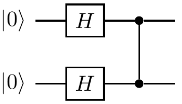
\includegraphics[width = 10em]{images/8.jpg}
\end{center}
Here are what happens:
\begin{itemize}
    \item \textbf{(After the Hadamard)} $$
    \Ket{00}\overset{H\otimes H}{\mapsto} \frac{1}{\sqrt{2}}(\Ket{0} + \Ket{1})\otimes\frac{1}{\sqrt{2}}(\Ket{0} + \Ket{1}) = \frac{1}{2}(\Ket{00} + \Ket{01} + \Ket{10} + \Ket{11})
    $$
    \item \textbf{(After the c-$P_\varphi$)} Recall what we did before: $\Ket{00} = \begin{bmatrix}
    1\\
    0\\
    0\\
    0
    \end{bmatrix}, \Ket{01} = \begin{bmatrix}
    0\\
    1\\
    0\\
    0
    \end{bmatrix}, \Ket{10} = \begin{bmatrix}
    0\\
    0\\
    1\\
    0
    \end{bmatrix}, \Ket{11} = \begin{bmatrix}
    0\\
    0\\
    0\\
    1
    \end{bmatrix}$, so we see that, operated by $
    \begin{bmatrix}
        1 & 0 & \vline & 0 & 0 \\
        0 & 1 & \vline & 0 & 0 \\
        \hline
        0 & 0 & \vline & 1 & 0 \\
        0 & 0 & \vline & 0 & e^{i\varphi} = e^{i\pi} = -1 \\
    \end{bmatrix},
    $ the only one that changes is $$
    \begin{bmatrix}
        1 & 0 & \vline & 0 & 0 \\
        0 & 1 & \vline & 0 & 0 \\
        \hline
        0 & 0 & \vline & 1 & 0 \\
        0 & 0 & \vline & 0 & -1 \\
    \end{bmatrix}\begin{bmatrix}
    0\\
    0\\
    0\\
    1
    \end{bmatrix} = -\begin{bmatrix}
    0\\
    0\\
    0\\
    1
    \end{bmatrix} = -\Ket{11}.
    $$ So, through the c-$P_\varphi$ gate at the end, we have $$
    \Ket{00} \overset{H\otimes H}{\mapsto} \frac{1}{2}(\Ket{00} + \Ket{01} + \Ket{10} + \Ket{11}) \overset{\text{c-}P_\varphi}{\mapsto} \frac{1}{2}(\Ket{00} + \Ket{01} + \Ket{10} - \Ket{11}),
    $$ which is an entangled state.
\end{itemize}

\subsection{General Controlled-$U$ Gate}
A generalization of controlled-$\NOT$ and controlled-$P_\varphi$ gates:
\begin{itemize}
    \item \textbf{(Matrix)} $$
    \text{Controlled-}U = \begin{bmatrix}
        1 & 0 & \vline & 0 & 0 \\
        0 & 1 & \vline & 0 & 0 \\
        \hline
        0 & 0 & \vline & U_{00} & U_{01} \\
        0 & 0 & \vline & U_{10} & U_{11} \\
    \end{bmatrix},
    $$ where $$
    U = \begin{bmatrix}
    U_{00} & U_{01} \\
    U_{10} & U_{11}
    \end{bmatrix}.
    $$
    \item \textbf{(Circuit)}
    \begin{center}
        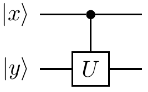
\includegraphics[width = 8em]{images/9.jpg}
    \end{center}
    \item \textbf{(Operator)} $$
    \text{c-}U = \kb{0}{0}\otimes \mathbb{1} + \kb{1}{1}\otimes U
    $$
\end{itemize}
\end{definition}

\begin{definition}[$x$-controlled-$U$ gate]
An even more general unitary operation that is an \hl{$x$-controlled-$U$ gate}, which can be formulated as: $$
\underset{x}{\sum}\kb{x}{x}\otimes U_x \equiv \kb{0}{0}\otimes U_0 + \kb{1}{1}\otimes U_1.
$$ This definition is more general in the sense that $\Ket{x}$ no longer needs to be $\Ket{0}$. In fact, $\Ket{x}\in \{0,1\}^n$, meaning it can be any arbitrary number of qubits. Similarly, $\Ket{y}\in \{0,1\}^m$. $U_x\in 2^m\times 2^n$ is applied to the second qubit whenever the first is in state $\Ket{x}$.
\end{definition}

\section{Universal Set of Gates}
We have seen many gates sand there are many more gates, but a universal set of gates is such that any unitary operations on any number of qubits can be constructed using gates from this set. One such universal set of gates using the gates we know so far is $$
\{H, S, \CNOT\},
$$ where $H$ is the Hadamard gate, $S = \begin{bmatrix}
    1 & 0\\
    0 & i
\end{bmatrix}$, and $\CNOT$ is controlled-$\NOT$.

\begin{proposition}
The bad news is, to approximate all possible circuits using only $\{H, S, \CNOT\}$ may lead to a \hl{$O(4^nn)$-blow-up}. But, if we only want to approximate to a precision of $\epsilon$, then the complexity is usually \hl{only polylog$\prt{\frac{1}{\epsilon}}$}.
\end{proposition}

\begin{remark}
Almost any gate that can entangle two qubits can be used as a universal gate. So, the above universal set of gates is far from a unique one. One particular example is $$
\{H, T = P_{\pi/4}, \CNOT\}.
$$
\end{remark}

\section{Phase Kick-Back}
This is an alternative way of introducing \textbf{phase shifts} that will be essential for our analysis of quantum algorithms.
\begin{definition}[Controlled-$U$ Interference]
It can be represented by the following circuit:
\begin{center}
    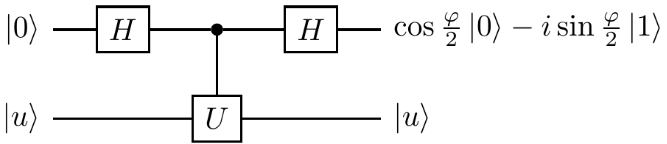
\includegraphics[width = 20em]{images/10.jpg},
\end{center}
where $\Ket{u}$ is an eigenstate of $U$, so that $U\Ket{u} = e^{i\varphi}\Ket{u}$ for some $\varphi$.
\end{definition}

\noindent We can write out the transformation steps:$$
\begin{aligned}
\Ket{0}\Ket{u}
\overset{H\otimes \mathbb{1}}{\mapsto}
& \frac{1}{\sqrt{2}}(\Ket{0}\Ket{u} + \Ket{1}\Ket{u})\\
\overset{\text{c-}U}{\mapsto}
& \frac{1}{\sqrt{2}}(\Ket{0}\Ket{u} + \Ket{1}U\Ket{u})\\
& = \frac{1}{\sqrt{2}}(\Ket{0} + \Ket{1}U)\Ket{u}\\
\end{aligned}
$$ Now, if $U$ is a \textbf{phase shift gate} by $\varphi$, we further have, ignoring constant factor ($\frac{1}{\sqrt{2}}$ and global phase factor) $$
\overset{H\otimes\mathbb{1}}{\mapsto}\prt{\cos\frac{\varphi}{2}\Ket{0} - i\sin\frac{\varphi}{2}\Ket{1}}\Ket{u}.
$$

\begin{remark}
Notice, in summary, what the circuit does is: $$
\boxed{\Ket{0}\Ket{u} \mapsto \prt{\cos\frac{\varphi}{2}\Ket{0} - i\sin\frac{\varphi}{2}\Ket{1}}\Ket{u}},
$$ which means that the second qubit is never changed, but the first qubit undergoes some phase shift. Now, this would be similar to what we had before for introducing \textbf{interference} on a single qubit, as the two circuits are very similar, and this may appear as a very complicated way of introducing phase shift. However, this is actually how quantum computers do it.
\end{remark}

\begin{example}\label{eg:x-ctrl-U}
Consider the following $x$-controlled-$U$ operation: $$
\begin{bmatrix}
1 & 0 & 0 & 0 \\
0 & 1 & 0 & 0 \\
0 & 0 & 1 & 0 \\
0 & 0 & 0 & X
\end{bmatrix} = \begin{tabular}{cc}
       & $\kb{00}{11}\otimes \mathbb{1}$ \\
   $+$ & $\kb{01}{01}\otimes \mathbb{1}$ \\
   $+$ & $\kb{10}{10}\otimes \mathbb{1}$ \\
   $+$ & $\kb{11}{11}\otimes X$ \\
\end{tabular}.
$$ In other words, nothing happens unless the first register is prepared in the $\Ket{11}$ state, in which case $X=\sigma_x$ is applied to flip the bit.\\

\noindent This unitary operation is a quantum version of the Boolean function, as $$
f(\Ket{xy}) = \begin{cases}
1\text{, if }\Ket{xy} = \Ket{11}\\
0\text{, otherwise}
\end{cases}
$$

\noindent We can also introduce the \textbf{phase kick-back mechanism} which introduces a relative phase in the equally-weighted superposition of all binary strings of length two: If we prepare the first register in superposition $$
\Ket{00} + \Ket{01} + \Ket{10} + \Ket{11},
$$, then the result of applying $x$-controlled-$U$ is $$
\Ket{00} + \Ket{01} + \Ket{10} - \Ket{11}.
$$ In other words, $X$ flips the bit and applies a phase factor of $e^{i\pi} = -1$ in front of teh corresponding term in the first register.
\end{example}

\begin{definition}[\textbf{phase kick-back mechanism}]
We have already introduced what \textbf{phase kick-back mechanism} means by the end of example \ref{eg:x-ctrl-U}. Here, we just note that \textbf{phase kick-back mechanism} is \hl{how we control quantum interference in quantum computation}.
\end{definition}

\section{Quick Words about Next Time}
Since there are entangled states: if we cannot attribute a state vector to an individual qubit, then how can we describe its quantum states? Answer: When our attentions are limited to a part of a larger system,
\begin{itemize}
    \item States are not represented by vectors.
    \item Measurements are not described by orthogonal projections.
    \item Evolution is not unitary.
\end{itemize}

\end{document}